\section{直线和圆的位置关系}

\subsection{直线和圆的联立}

\begin{theorem}
    令两交点坐标为 $A(x_1, y_1)$ 和 $B(x_2, y_2)$，则可利用韦达定理得到 $x_1 + x_2$ 和 $x_1 \cdot x_2$.

    通过联立方程，可以消去 $y$，得到关于 $x$ 的一元二次方程 $ax^2 + bx + c = 0$，则有：
    $$x_1 + x_2 = -\frac{b}{a} \quad x_1 \cdot x_2 = \frac{c}{a}$$
    类似地，也可以得到 $y_1 + y_2$ 和 $y_1 \cdot y_2$。
\end{theorem}

\begin{example}
    联立直线 $y = kx + b$ 与圆 $(x-a)^2 + (y-c)^2 = r^2$ 的方程：
    \begin{align}
        \begin{cases}
            y = kx + b \\
            (x-a)^2 + (y-c)^2 = r^2
        \end{cases}
    \end{align}
\end{example}

\begin{solution}
    将直线方程代入圆的方程：
    \begin{align}
        (x-a)^2 + (kx+b-c)^2 - r^2 & = 0
    \end{align}

    展开得到关于 $x$ 的一元二次方程：
    \begin{align}
        (1+k^2)x^2 + 2(-a+k(b-c))x + (a^2+(b-c)^2-r^2) & = 0
    \end{align}

    \begin{center}
        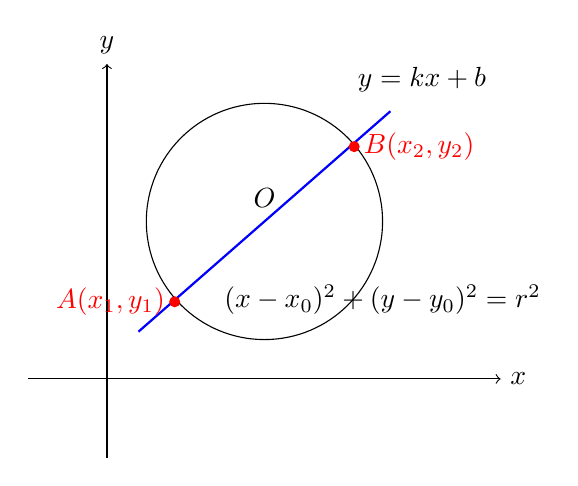
\begin{tikzpicture}[scale=1]
            % Draw coordinate axes
            \draw[->] (-1,0) -- (5,0) node[right] {$x$};
            \draw[->] (0,-1) -- (0,4) node[above] {$y$};

            % Draw the circle
            \draw (2,2) circle (1.5);
            \node at (2,2.3) {$O$};
            % Draw the line - extended on both sides
            \draw[blue, thick] (0.4,0.6) -- (3.6,3.4);

            % Mark the intersection points
            \fill[red] (0.86,0.98) circle (2pt) node[left] {$A(x_1,y_1)$};
            \fill[red] (3.14,2.95) circle (2pt) node[right] {$B(x_2,y_2)$};

            % Label the circle and line
            \node at (3.5,1) {$(x-x_0)^2+(y-y_0)^2=r^2$};
            \node at (4,3.8) {$y=kx+b$};
        \end{tikzpicture}
    \end{center}
\end{solution}

\subsection{直线和圆的交点个数}

\begin{theorem}[直线和圆的交点个数]
    直线 $A x+B y+C=0$ 与圆 $(x-a)^2+(y-b)^2=r^2$ 的位置关系有三种：
    \begin{itemize}
        \item $d>r \Leftrightarrow$ 相离 $\Leftrightarrow \Delta<0$ ；
        \item $d=r \Leftrightarrow$ 相切 $\Leftrightarrow \Delta=0$ ；
        \item $d<r \Leftrightarrow$ 相交 $\Leftrightarrow \Delta>0$ ．
    \end{itemize}
    其中：
    $$d=\frac{|A a+B b+C|}{\sqrt{A^2+B^2}}$$
\end{theorem}

\subsection{向量式}

\begin{theorem}[向量式]
    联立利用韦达定理求出两交点横坐标之积 $x_M x_N$，再结合向量点积的坐标表示 $\overrightarrow{O M} \cdot \overrightarrow{O N} = x_M x_N + y_M y_N$ 求解。

    \begin{warning}
        求出 $y_M y_N$ 和 $y_M + y_N$ 的方法是代入直线中，相乘和相加即可：
        $$
            \begin{cases}
                y_M = kx_M + b \\
                y_N = kx_N + b
            \end{cases}
        $$
    \end{warning}
\end{theorem}

\begin{example}
    直线 $y=k x$ 与圆 $(x-1)^2+(y-1)^2=1$ 交于 $M 、 N$ 两点，$O$ 为坐标原点，则 $\overrightarrow{O M} \cdot \overrightarrow{O N}=$（ \hspace{2em} ）
    \begin{tasks}(4)
        \task $\frac{1}{1+k^2}$
        \task $\frac{k^2}{1+k^2}$
        \task $1$
        \task $2$
    \end{tasks}
\end{example}

\v{15em}

\begin{example}
    已知圆 $C$ 的半径为 2 ，圆心在 $x$ 轴正半轴上，直线 $3 x-4 y+4=0$ 与圆 $C$ 相切．
    \begin{enumerate}
        \item 求圆 $C$ 的方程；$(x-2)^2+y^2=4$
        \item 若过点 $(0,-3)$ 的直线 $l$ 与圆 $C$ 交于不同的两点 $A, B$ ，且 $\overrightarrow{O A} \cdot \overrightarrow{O B}=3, O$ 为坐标原点，求 $\triangle A O B$ 的面积．
    \end{enumerate}
\end{example}

\vspace{10em}

\subsection{弦长公式}

\begin{theorem}[弦长公式]
    设直线和圆的两个交点为 $A(x_1, y_1), B(x_2, y_2)$，圆心为 $O$，则弦长 $L$ 满足
    \[
        L = \sqrt{(x_2 - x_1)^2 + (y_2 - y_1)^2}
    \]
    设这条直线的斜率是 $k$，则：
    $$
        L = \sqrt{1+k^2}|x_1-x_2| = \sqrt{1+k^2}\sqrt{(x_1+x_2)^2-4x_1x_2}
    $$
    如果联立时采用的是 $y_1$ 和 $y_2$，则：
    $$
        L = \sqrt{1+\frac{1}{k^2}}|y_1-y_2| = \sqrt{1+\frac{1}{k^2}}\sqrt{(y_1 + y_2)^2 - 4y_1y_2}
    $$
\end{theorem}

\begin{example}
    $y=x+4$ 与 $C:(x-1)^2+(y-3)^2=8$ 交于 $M, ~ N$，$O$ 为原点，则 $|M N|=$ \underline{\qquad} , $\overrightarrow{O M} \cdot \overrightarrow{O N}=$ \underline{\qquad}
\end{example}

\v{12em}

\begin{example}
    已知直线 $l: k x-y+5=0$ ，圆 $C: x^2+y^2-6 x-4 y-12=0$ ．
    \begin{enumerate}
        \item 当 $k=2$ 时，判断直线 $l$ 与圆 $C$ 的位置关系；
        \item 记直线 $l$ 与圆 $C$ 的交点为 $A, B$ ，当 $|A B|=2 \sqrt{7}$ 时，求 $k$ 的值．
    \end{enumerate}
\end{example}

\vspace{10em}

\subsection*{联立训练}

\begin{example}
    已知过点 $A(0,1)$ 且斜率为 $k$ 的直线 $l$ 与圆 $C:(x-2)^2+(y-3)^2=1$ 交于点 $M$、$N$ 两点．
    \begin{enumerate}
        \item 求 $k$ 的取值范围；
        \item 若 $\overrightarrow{O M} \cdot \overrightarrow{O N}=12$ ，其中 $O$ 为坐标原点，求 $|M N|$ ．
    \end{enumerate}
\end{example}

\v{12em}

\begin{example}
    设 $O$ 是坐标原点，直线 $x+2 y-3=0$ 与圆 $C: x^2+y^2+x-6 y+m=0$ 交于 $P, Q$ 两点．
    \begin{itemize}
        \item[（1）] 求线段 $P Q$ 中点 $M$ 的坐标；
        \item[（2）] 若 $O P \perp O Q$ ，求该圆的面积．
    \end{itemize}
\end{example}

\v{12em}

\begin{example}
    已知斜率为 $k\left(k \neq-\frac{1}{2}\right)$ 的直线 $l$ 过点 $B(-2,0)$ ，圆 $A:(x+1)^2+(y-2)^2=20$ 与 $l$ 交于 $M, N$ 两点，线段 $M N$ 中点是 $Q$.
    \begin{itemize}
        \item[（1）] 若 $k=1$ ，求 $Q$ 坐标
        \item[（2）] 若直线 $l_1: x+2 y+7=0$ 与直线 $l$ 交点是 $P$ ，那么 $\overrightarrow{B P} \cdot \overrightarrow{B Q}$ 是否为定值？如果是，求出定值；如果不是，说明理由．
    \end{itemize}
\end{example}

\begin{tips}
    因为 Q 是中点，根据垂径定理，可以拆成 $\overrightarrow{BQ}= \overrightarrow{BA}+\overrightarrow{AQ}$，然后利用垂直就变了 $\overrightarrow{BA} \cdot \overrightarrow{BP}$.
\end{tips}

\v{12em}

\pagebreak

\begin{theorem}[以 AB 为直径的圆过某点]
    设圆上一点为 $K$，则有 $\overrightarrow{KM} \cdot \overrightarrow{KN} = 0$（直径所对的圆周角是直角）.
    \begin{center}
        \begin{tikzpicture}[scale=0.8]
            % Coordinate axes
            \draw[->] (-3,0) -- (3,0) node[right] {$x$};
            \draw[->] (0,-2) -- (0,3) node[above] {$y$};

            % Circle with center O
            \coordinate (O) at (0,0);
            \draw (O) circle (2);
            \fill (O) circle (1.5pt) node[below right] {$O$};

            % Points M and N (diameter endpoints)
            \fill[blue] (-2,0) circle (2pt) node[below left] {$M$};
            \fill[blue] (2,0) circle (2pt) node[below right] {$N$};

            % Point K on the circle (perpendicular to diameter)
            \fill[red] (0,2) circle (2pt) node[above right] {$K$};

            % Connect lines
            \draw[thick] (-2,0) -- (2,0);  % MN (diameter)
            \draw[dashed] (0,2) -- (-2,0);   % KM
            \draw[dashed] (0,2) -- (2,0);   % KN

            % Right angle mark at K
            \draw (0.3,1.7) -- (0,1.4) -- (-0.3,1.7);

            % Label for the theorem
            \node at (0,-2.5) {以 $MN$ 为直径的圆中，$K$ 处的圆周角为直角};
        \end{tikzpicture}
    \end{center}
\end{theorem}

\begin{example}
    已知圆 $C$ 经过 $P(4,-2), Q(-1,3)$ 两点，且圆心 $C$ 在直线 $x+y-1=0$ 上．
    \begin{itemize}
        \item[（1）] 求圆 $C$ 的方程；
        \item[（2）] 若直线 $l: y=-x+m$ 与圆 $C$ 交于点 $A, B$ ，且以线段 $A B$ 为直径的圆经过坐标原点，求直线 $l$ 的方程．
    \end{itemize}
\end{example}

\v{12em}

\subsection{直线与圆的交点弦长取值范围}

\begin{theorem}[直线与圆的交点的弦长取值范围]
    然后利用圆心到直线的距离 $d$、半径 $r$ 和弦长 $L$ 之间的关系 $L=2\sqrt{r^2-d^2}$。
\end{theorem}

\begin{example}
    已知直线 $l:(m-1) x+2 y+3-m=0$ 与圆 $C: x^2+y^2-6 x+6 y=0$ 交于 $A, B$ 两点，则线段 $A B$ 的长度的取值范围是（ \hspace{2em} ）
    \begin{tasks}(4)
        \task $[\sqrt{10}, 3 \sqrt{2}]$
        \task $[2 \sqrt{10}, 6 \sqrt{2}]$
        \task $[2 \sqrt{10}, 4 \sqrt{2}]$
        \task $[\sqrt{10}, 6 \sqrt{2}]$
    \end{tasks}
\end{example}

\v{12em}

\subsection{直线与圆的距离最值}

\begin{theorem}[点到直线的距离与圆的几何性质]
    求圆上动点与固定两点构成三角形面积的最值问题，通常转化为求圆上动点到该固定两点所在直线的距离的最值问题。其最小（大）距离等于圆心到直线的距离减（加）去半径。
\end{theorem}

\begin{example}
    已知两点 $A(-1,0), ~ B(0,2)$ ，点 $P$ 是圆 $(x-2)^2+y^2=1$ 上任意一点，则 $\triangle P A B$ 面积的最小值是（ \hspace{2em} ）
    \begin{tasks}(4)
        \task $\sqrt{5}$
        \task $2$
        \task $3+\frac{\sqrt{5}}{2}$
        \task $3-\frac{\sqrt{5}}{2}$
    \end{tasks}
\end{example}

\vspace{10em}

\subsection{半圆}

\begin{theorem}
    如果一个圆的方程中出现了根号，需要注意定义域，此时的圆可能是一个半圆。

    例如，$y = \sqrt{1-x^2}$ 表示的是半径为 1 的半圆，其中 $x \in [-1, 1]$，$y \geq 0$。

    同理，$y = -\sqrt{1-x^2}$ 表示下半圆，$x = \sqrt{1-y^2}$ 表示右半圆，$x = -\sqrt{1-y^2}$ 表示左半圆。

    \begin{center}
        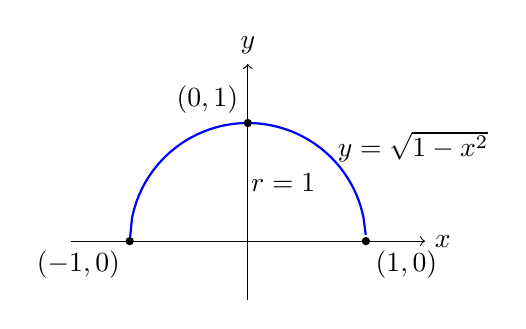
\begin{tikzpicture}[scale=1.5]
            \draw[->] (-1.5,0) -- (1.5,0) node[right] {$x$};
            \draw[->] (0,-0.5) -- (0,1.5) node[above] {$y$};

            \draw[thick, blue, domain=-1:1, samples=100] plot (\x, {sqrt(1-\x*\x)});

            \fill (-1,0) circle (1pt) node[below left] {$(-1,0)$};
            \fill (1,0) circle (1pt) node[below right] {$(1,0)$};
            \fill (0,1) circle (1pt) node[above left] {$(0,1)$};

            \node at (1.4,0.8) {$y = \sqrt{1-x^2}$};

            \draw[dashed] (0,0) -- (0,1);
            \node at (0.3,0.5) {$r=1$};
        \end{tikzpicture}
    \end{center}

    在处理含有根号的圆方程时，必须考虑其定义域限制，并确定图形是完整的圆还是部分圆弧。
\end{theorem}

\begin{example}
    \begin{enumerate}
        \item 已知过 $(-3,0)$ 的直线与曲线 $y=\sqrt{1-x^2}$ 相切，求该直线的方程。
        \item 求满足曲线 $y=\sqrt{1-x^2}$ 上的点 $(x,y)$ 与 $(4,0)$ 点形成的斜率的取值范围。
    \end{enumerate}
\end{example}

\vspace{10em}

\begin{example}
    已知直线 $l: x+2 y+t=0$ ，曲线 $C: y=\sqrt{4-x^2}$ ，则＂$l$ 与 $C$ 相切＂是＂$t=2 \sqrt{5}$＂的 （\qquad）
    \begin{tasks}(4)
        \item 充分不必要条件
        \item 充分必要条件
        \item 不充分也不必要条件
        \item 必要非充分条件
    \end{tasks}
\end{example}

\v{12em}

\subsection{圆上有几个点到直线的距离}

\begin{theorem}
    需要分为直线和圆是否相交、相切、相离三种情况来讨论。
    \begin{center}
        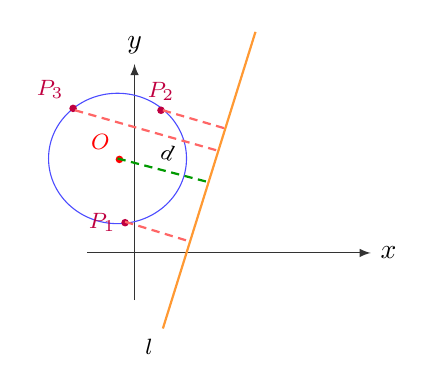
\begin{tikzpicture}[scale=1.2]
            % Coordinate axes
            \draw[draw=black!80, -latex, thin] (-2.00,0.00) -- (1.00,0.00) node[right] {$x$};
            \draw[draw=black!80, -latex, thin] (-1.50,-0.50) -- (-1.50,2.00) node[above] {$y$};

            % Circle
            \draw[draw=blue!70, thin] (-1.68,1.00) ellipse (0.73 and 0.69);
            \fill[red] (-1.66,0.99) circle (0.04) node[anchor=south east, font=\footnotesize] {$O$};

            % Line
            \draw[draw=orange!80, thin, thick] (-0.22,2.34) -- (-1.20,-0.80) node[below left, font=\footnotesize] {$l$};

            % Distance from center to line
            \draw[draw=green!60!black, thick, densely dashed] (-1.68,1.00) -- (-0.72,0.75)
            node[midway, above, font=\footnotesize, sloped] {$d$};

            % Points on the circle
            \fill[purple] (-1.60,0.32) circle (0.04) node[left, font=\footnotesize] {$P_1$};
            \fill[purple] (-1.22,1.51) circle (0.04) node[above, font=\footnotesize] {$P_2$};
            \fill[purple] (-2.15,1.53) circle (0.04) node[above left, font=\footnotesize] {$P_3$};

            % Distance lines
            \draw[draw=red!60, thick, densely dashed] (-1.60,0.33) -- (-0.91,0.12);
            \draw[draw=red!60, thick, densely dashed] (-1.20,1.51) -- (-0.55,1.32);
            \draw[draw=red!60, thick, densely dashed] (-2.13,1.51) -- (-0.61,1.08);
        \end{tikzpicture}
    \end{center}
\end{theorem}

\v{2em}

\begin{example}
    已知圆 $C:(x+1)^2+y^2=4$ ．
    \begin{enumerate}
        \item 过点 $P(1,3)$ 作圆的切线，求切线 $l$ 的方程；
        \item 已知圆 $C^{\prime}:(x+1)^2+y^2=r^2$ 上只有 2 个点到直线 $l^{\prime}: 4 x-3 y-6=0$ 的距离为 1 ，求 $r$ 的取值范围．
    \end{enumerate}
\end{example}

\vspace{10em}

\begin{example}
    ＂$3<r<6$＂是＂圆 $C:(x+1)^2+(y-2)^2=r^2(r>0)$ 上
    恰有 2 个点到直线 $l: 3 x+4 y+15=0$ 的距离为 1 ＂的（\quad ）条件（填是否充分必要）
\end{example}

\v{10em}

\begin{problemset}
    \item 已知圆 $C: x^2-4 x+y^2=0$ 直线 $l:(m+1) x+2 y-3-m=0,(m \in \mathbf{R})$ ，则 （\qquad）
    \begin{tasks}
        \task 直线恒过定点 $(1,1)$
        \task 存在实数 $m$ ，使得直线 $l$ 与圆 $C$ 没有公共点
        \task 当 $m=-3$ 时，圆 $C$ 上恰有两个点到直线 $r$ 的距离等于 1
        \task 圆 $C$ 与圆 $x^2+y^2-2 x+8 y+1=0$ 只有一条公切线
    \end{tasks}

    \item 圆 $C: x^2+y^2-2 x=0$ 和圆 $D: x^2+y^2+2 x-4 y=0$ 的交点为 $A, B$ ，则有 （\qquad）
    \begin{tasks}
        \task 公共弦 $A B$ 所在直线方程为 $x-y=0$
        \task 过直线 $A B$ 上任意一点 $P$ 作圆 $(x+3)^2+(y-1)^2=1$ 的切线，切于点 $Q$ ，则$|P Q|$ 的最小值为 $\sqrt{7}$
        \task 公共弦 $A B$ 的长为 $\frac{\sqrt{2}}{2}$
        \task 圆 $N$ ：$(x+1)^2+(y-2)^2=1$ 与圆 $C$ 关于直线 $x-y+1=0$ 对称
    \end{tasks}

    \item 已知直线 $l:(2+t) x-(1+t) y-12-8 t=0, ~ Q$ 是圆 $O: x^2+y^2=4$ 上的一动点，则点 $Q$ 到直线 $l$ 的距离 $d$ 的取值范围为 （\qquad）
    \begin{tasks}(4)
        \task $[0,4 \sqrt{2}-2]$
        \task $[0,4 \sqrt{2}+2)$
        \task $[0,4 \sqrt{2}+2]$
        \task $[1,4 \sqrt{2}-2)$
    \end{tasks}

    \item 已知圆 $C_1: x^2+y^2-2 x-4 y-7=0$ 和圆 $C_2:(x+3)^2+(y+1)^2=12$ 交于两点，点 $P$ 在圆 $C_1$ 上运动，点 $Q$ 在圆 $C_2$ 上运动，则下列说法正确的是 （\qquad）
    \begin{tasks}
        \task 圆 $C_1$ 和圆 $C_2$ 关于直线 $8 x+6 y-5=0$ 对称
        \task 圆 $C_1$ 和圆 $C_2$ 的公共弦长为 $2 \sqrt{23}$
        \task $|P Q|$ 的取值范围为 $[0,5+2 \sqrt{3}]$
        \task 若 $M$ 为直线 $x-y+8=0$ 上的动点，则 $|P M|+|M Q|$ 的最小值为 $\sqrt{109}-4 \sqrt{3}$
    \end{tasks}

    \item $M$ 是抛物线 $y^2=x$ 上一点，$N$ 是圆 $C:(x+1)^2+(y-4)^2=1$ 关于直线 $x-y+1=0$ 的对称圆 $C$ 上的一点，则 $|M N|$ 的最小值是 \underline{\qquad}.
\end{problemset}

\begin{tips}
    \begin{enumerate}
        \item AC.
              \begin{enumerate}
                  \item 对于 $A$ ，直线 $l$ 的方程为 $(x-1) m+x+2 y-3=0$ ，由 $\left\{\begin{array}{l}x-1=0 \\ x+2 y-3=0\end{array}\right.$ ，得 $\left\{\begin{array}{l}x=1 \\ y=1\end{array}\right.$ ，直线 $l$ 过定点 $(1,1)$ ，故A正确；
                  \item 对于 $B$ ，$C:(x-2)^2+y^2=4$ ，又 $(1-2)^2+1^2=2<4$ ，即定点 $(-1,1)$ 在圆 $C$ 内，则直线 $l$ 与圆 $C$ 相交，有两个交点，故 $B$ 错误；
                  \item 对于 $C$ ，当 $m=-3$ 时，直线 $l: x-y=0$ ，圆心 $C(2,0)$ 到直线 $l$ 的距离为 $d=\frac{|2-0|}{\sqrt{2}}=\sqrt{2}$ ，
                        而圆 $C$ 半径为 2 ，且 $2-\sqrt{2}<1$ ，因此恰有 2 个点到直线 $l$ 的距离等于 1 ，故C正确；
                  \item 对于D，圆 $x^2+y^2-2 x+8 y+1=0$ 化为 $(x-1)^2+(y+4)^2=16$ ，
                        圆 $x^2+y^2-2 x+8 y+1=0$ 的圆心为 $(1,-4)$ ，半径为 4 ，
                        两圆圆心距为 $4-2=2<d=\sqrt{(1-2)^2+(-4-0)^2}=\sqrt{17}<6=4+2$ ，

                        所以两圆相交，因此它们有两条公切线，故 $D$ 错误．
              \end{enumerate}

        \item \begin{enumerate}
                  \item 对于A，将两圆方程相减即可；
                  \item 对于 B ，切线段长 $P Q=\sqrt{P M^2-r_M^2}$ ，圆 $M$ 半径 $r_M$ 为定值，故令 $P M$ 最小即可，而 $P M$ 的最小值，就是 $M$ 到直线 $A B$ 的距离；
                  \item 对于 C ，求出圆 $C$ 或圆 $D$ 的圆心到直线 $A B$ 的距离 $d$ ，利用圆的弦长公式 $A B=2 \sqrt{r^2-d^2}$ 求解即可；
                  \item 对于D，判断两圆半径是否相同，圆心是否关于直线对称即可．
              \end{enumerate}
        \item 选B. 直线 $l:(2+t) x-(1+t) y-12-8 t=0$ ，可化为：
              $$
                  (x-y-8) t+2 x-y-12=0
              $$
              由 $\left\{\begin{array}{c}2 x-y-12=0 \\ x-y-8=0\end{array}\right.$ ，解得 $x=4, ~ y=-4$ ，所以 $l$ 过定点 $P(4,-4)$ ，

              又因为点 $Q$ 在圆 $O$ 上，且 $|O P|=4 \sqrt{2}$ ，圆 $O$ 的圆心为 $O(0,0)$ ，半径 $r=2$，

              所以当 $O P \perp l$ ，且 $Q, ~ O, ~ P$ 三点共线时，点 $Q$ 到直线 $l$ 的距离 $d$ 最大，最大为 $4 \sqrt{2}+2$ ，此时 $k_{O P}=\frac{-4-0}{4-0}=-1$ ，所以直线 $l$ 的斜率为 1 ，即 $2+t=1+t$ ，无解，

              故直线 $l$ 不存在，所以 $d<4 \sqrt{2}+2$ ；

              当直线 $l$ 与圆 $O$ 相交或相切时，点 $Q$ 到直线 $l$ 的距离 $d$ 最小，最小为 0 ，

              故点 $Q$ 到直线 $l$ 的距离 $d$ 的取值范围为 $[0,4 \sqrt{2}+2)$ ．
        \item 选D.
              \begin{enumerate}
                  \item 对于 $\mathrm{A}, ~ C_1: x^2+y^2-2 x-4 y-7=0$ 和圆 $C_2:(x+3)^2+(y+1)^2=12$ ，圆心和半径分别是 $C_1(1,2), C_2(-3,-1), R_1=2 \sqrt{3}, R_2=2 \sqrt{3}$ ，则两圆心中点为 $\left(-1, \frac{1}{2}\right)$

                        若圆 $C_1$ 和圆 $C_2$ 关于直线 $8 x+6 y-5=0$ 对称，则直线是 $C_1 C_2$ 的中垂线，但两圆心中点 $\left(-1, \frac{1}{2}\right)$ 不在直线 $8 x+6 y-5=0$ 上，故A错误；

                  \item 对于 $\mathrm{B}, ~ C_1$ 到直线 $8 x+6 y+5=0$ 的距离 $d=\frac{|8+12+5|}{10}=\frac{5}{2}$ ，故公共弦长为 $2 \sqrt{(2 \sqrt{3})^2-\left(\frac{5}{2}\right)^2}=\sqrt{23}$ ，B错误；

                  \item 对于 C ，圆心距为 $\sqrt{(1+3)^2+(2+1)^2}=5$ ，当点 $P$ 和 $Q$ 重合时，$|P Q|$ 的值最小，当 $P, Q, C_1, C_2$ 四点共线时，$|P Q|$ 的值最大为 $5+4 \sqrt{3}$ ，
                        故 $|P Q|$ 的取值范围为 $[0,5+4 \sqrt{3}], ~ C$ 错误；

                  \item 对于 D ，如图，设 $C_1$ 关于直线 $x-y+8=0$ 对称点为 $A(m, n)$ ，

                        则 $\left\{\begin{array}{c}\frac{2-n}{1-m}=-1, \\ \frac{m+1}{2}-\frac{n+2}{2}+8=0,\end{array}\right.$ 解得 $\left\{\begin{array}{c}m=-6, \\ n=9,\end{array}\right.$

                        即 $C_1$ 关于直线 $x-y+8=0$ 对称点为 $A(-6,9)$ ，
                        连接 $A C_2$ 交直线于点 $M$ ，此时 $|P M|+|M Q|$ 最小，
                        $$
                            |P M|+|M Q| \geq\left|M C_1\right|+\left|M C_2\right|-4 \sqrt{3}=\left|C_2 A\right|-4 \sqrt{3}=\sqrt{(-6+3)^2+(9+1)^2}-4 \sqrt{3}=\sqrt{109}-4 \sqrt{3},
                        $$
                        即 $|P M|+|M Q|$ 的最小值为 $\sqrt{109}-4 \sqrt{3}$ ，D正确．
              \end{enumerate}
    \end{enumerate}
\end{tips}